\documentclass{dlproblemset}
\usepackage{tikz}
\usetikzlibrary{positioning}
\tikzset{every picture/.style={line width=0.75pt}}

% ---- Nodos de grafo computacional usados na questão do backward do nodo de dropout ----
% Mesma convenção da aula: variáveis em círculo, operações em caixa,
% gradientes anotados abaixo de cada aresta.
\tikzset{
  cgvar/.style  ={circle, draw=black, minimum size=0.8cm, inner sep=1pt, font=\small},
  cgopw/.style  ={rectangle, rounded corners=2pt, draw=black, fill=black!8,
                  minimum height=0.8cm, inner sep=4pt, font=\small},
  cgedge/.style ={->, >=stealth, thick, gray!70},
  cggrad/.style ={font=\scriptsize, fill=white, inner sep=1.5pt},
}

\title{Softmax, Entropia Cruzada e Grafo Computacional}
\subtitle{Lista de Exercícios}

\begin{document}

\begin{enumerate}[1)]

    \item Em um grafo computacional, o \textit{backward pass} percorre o grafo na ordem inversa aplicando a regra da cadeia localmente em cada nodo. Para calcular o gradiente que envia às suas arestas de entrada, o que cada nodo precisa conhecer?
    \begin{enumerate}[(a)]
        \item O gradiente \textit{upstream} que chega pela sua saída e a derivada local da sua operação em relação a cada entrada.
        \item A expressão simbólica completa da função representada pelo grafo e a derivada algébrica dela em relação a cada folha.
        \item O valor da \textit{loss} avaliada duas vezes, com cada entrada perturbada por um passo $h$, para estimar a derivada por diferença finita.
        \item O gradiente da \textit{loss} em relação a todos os parâmetros da rede, obtido antes do início do percurso na ordem inversa.
    \end{enumerate}
    %a

    \item Considere o grafo computacional da função $f(a,b,c) = (a + b)\cdot(b \cdot c)$, com nodos intermediários $u = a + b$ e $v = b \cdot c$. Note que a variável $b$ alimenta dois nodos do grafo. Para $a = 1$, $b = 2$ e $c = 3$, após o \textit{forward pass} e o \textit{backward pass} iniciado com $\partial f / \partial f = 1$, qual o valor de $\partial f / \partial b$?
    \begin{enumerate}[(a)]
        \item $6$
        \item $9$
        \item $15$
        \item $18$
    \end{enumerate}
    %c

    \item Considere a função $f(a,b,c) = (a + b)\cdot\max(b, c)$, decomposta em um grafo computacional com três nodos de operação: $u = a + b$ (nodo de soma), $v = \max(b, c)$ (nodo de máximo) e $f = u \cdot v$ (nodo de produto). Repare que a variável $b$ alimenta dois nodos. Para $a = 2$, $b = 3$ e $c = 4$, resolva os itens abaixo:
    \begin{enumerate}[a)]
        \item Compute o \textit{forward pass}, informando o valor de cada nodo intermediário e da saída $f$.
        \item Compute o \textit{backward pass} nodo a nodo, iniciando com $\partial f/\partial f = 1$, e informe os gradientes $\partial f/\partial a$, $\partial f/\partial b$ e $\partial f/\partial c$. Indique, em cada nodo, qual padrão foi aplicado (distribuidor, comutador ou roteador) e como os gradientes que chegam em $b$ são combinados.
    \end{enumerate}

    \item A regressão logística $\hat{y} = \sigma(\theta_0 + \theta_1 x_1 + \theta_2 x_2)$, treinada com a \textit{Binary Cross Entropy} $L = -\bigl(y\ln\hat{y} + (1-y)\ln(1-\hat{y})\bigr)$, pode ser vista como um grafo computacional. Resolva os itens abaixo:
    \begin{enumerate}[a)]
        \item Decomponha a computação de $L$ em nodos elementares, explicitando os nodos de produto, os nodos de soma, o nodo sigmoide (já agrupado em uma única operação, como visto em aula) e o nodo da \textit{loss}.
        \item Derive $\partial L/\partial \theta_0$, $\partial L/\partial \theta_1$ e $\partial L/\partial \theta_2$ aplicando a regra da cadeia nodo a nodo, no sentido inverso do grafo, informando o gradiente que atravessa cada nodo. Simplifique as expressões finais.
    \end{enumerate}

    \item \textit{Frameworks} como PyTorch representam a computação como um grafo construído automaticamente durante a execução do código \textit{forward}, e é esse grafo que permite calcular as derivadas automaticamente, como discutido em aula. Explique por que essa representação é necessária para o cálculo automático de gradientes e descreva o que precisa ser armazenado durante o \textit{forward pass} para que o \textit{backward pass} seja possível. Ilustre com pelo menos dois nodos concretos cujas derivadas locais dependem de valores calculados no \textit{forward}.

    \item No nodo de produto de matrizes $\mathbf{Z} = \mathbf{A}\,\mathbf{\Theta}^{\top}$, visto na versão vetorizada do grafo computacional, temos $\mathbf{A} \in \mathbb{R}^{N\times d_e}$, $\mathbf{\Theta} \in \mathbb{R}^{d_s\times d_e}$, e o \textit{backward} recebe o gradiente \textit{upstream} $\mathbf{G} = \partial J/\partial \mathbf{Z} \in \mathbb{R}^{N\times d_s}$. Quais expressões computam os gradientes das duas entradas do nodo?
    \begin{enumerate}[(a)]
        \item $\partial J/\partial \mathbf{A} = \mathbf{G}\,\mathbf{\Theta}$ e $\partial J/\partial \mathbf{\Theta} = \mathbf{G}^{\top}\mathbf{A}$.
        \item $\partial J/\partial \mathbf{A} = \mathbf{G}\,\mathbf{\Theta}^{\top}$ e $\partial J/\partial \mathbf{\Theta} = \mathbf{A}^{\top}\mathbf{G}$.
        \item $\partial J/\partial \mathbf{A} = \mathbf{G}^{\top}\mathbf{A}$ e $\partial J/\partial \mathbf{\Theta} = \mathbf{G}\,\mathbf{\Theta}$.
        \item $\partial J/\partial \mathbf{A} = \mathbf{\Theta}^{\top}\mathbf{G}$ e $\partial J/\partial \mathbf{\Theta} = \mathbf{A}\,\mathbf{G}^{\top}$.
    \end{enumerate}
    %a

    \item Considere o MLP vetorizado representado como grafo computacional com os nodos \textit{matmul}, sigmoide e \textit{loss}, como visto em aula: $\mathbf{Z}^{(1)} = \mathbf{X}{\mathbf{\Theta}^{(1)}}^{\top}$, $\mathbf{A}^{(1)} = \sigma(\mathbf{Z}^{(1)})$, $\mathbf{Z}^{(2)} = \mathbf{A}^{(1)}{\mathbf{\Theta}^{(2)}}^{\top}$, $\hat{y} = \sigma(\mathbf{Z}^{(2)})$ e $J = \tfrac{1}{2}\sum\left(y - \hat{y}\right)^{2}$. Use uma única observação $\mathbf{X} = \begin{bmatrix} 1 & 2 \end{bmatrix}$ com alvo $y = 1$ e pesos
    $$\mathbf{\Theta}^{(1)} = \begin{bmatrix} 0.5 & -0.5 \\ 0.5 & 0.5 \end{bmatrix}, \qquad \mathbf{\Theta}^{(2)} = \begin{bmatrix} 0.5 & -0.5 \end{bmatrix}.$$
    \begin{enumerate}[a)]
        \item Execute o \textit{forward pass} nodo a nodo, informando $\mathbf{Z}^{(1)}$, $\mathbf{A}^{(1)}$, $\mathbf{Z}^{(2)}$, $\hat{y}$ e $J$.
        \item Execute o \textit{backward pass} nodo a nodo, iniciando com $\partial J/\partial J = 1$, informando o gradiente na saída de cada nodo e, ao final, $\partial J/\partial \mathbf{\Theta}^{(1)}$ e $\partial J/\partial \mathbf{\Theta}^{(2)}$. Em cada passo, indique qual regra de \textit{backward} foi aplicada (nodo \textit{loss}, nodo de ativação ou nodo \textit{matmul}).
    \end{enumerate}

    \item Os dois nodos vetorizados abaixo foram vistos em aula. Em ambos, $\mathbf{G}$ é o gradiente \textit{upstream} que chega pela saída do nodo, e as expressões anotadas abaixo das arestas de entrada são os gradientes que o nodo envia para trás.

    \begin{center}
    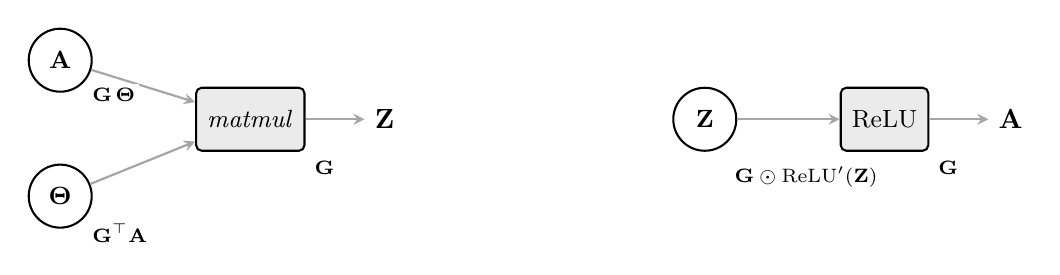
\begin{tikzpicture}[node distance=0.9cm and 1.3cm]
        % nodo matmul
        \node[cgvar] (A) {$\mathbf{A}$};
        \node[cgvar, below=of A] (T) {$\mathbf{\Theta}$};
        \node[cgopw, right=of A, yshift=-0.75cm] (mm) {\textit{matmul}};
        \node[right=of mm, xshift=-0.55cm] (Z) {$\mathbf{Z}$};
        \draw[cgedge] (A) -- (mm);
        \draw[cgedge] (T) -- (mm);
        \draw[cgedge] (mm) -- (Z);
        \node[cggrad, below right=0.05cm and 0.05cm of mm] {$\mathbf{G}$};
        \node[cggrad, below right=0.0cm and 0.05cm of A] {$\mathbf{G}\,\mathbf{\Theta}$};
        \node[cggrad, below right=0.0cm and 0.05cm of T] {$\mathbf{G}^{\top}\mathbf{A}$};
        % nodo ReLU
        \node[cgvar, right=3.4cm of Z] (Z2) {$\mathbf{Z}$};
        \node[cgopw, right=of Z2] (rl) {ReLU};
        \node[right=of rl, xshift=-0.55cm] (A2) {$\mathbf{A}$};
        \draw[cgedge] (Z2) -- (rl);
        \draw[cgedge] (rl) -- (A2);
        \node[cggrad, below right=0.05cm and 0.05cm of rl] {$\mathbf{G}$};
        \node[cggrad, below right=0.24cm and 0.02cm of Z2] {$\mathbf{G} \odot \mathrm{ReLU}'(\mathbf{Z})$};
    \end{tikzpicture}
    \end{center}

    O nodo de \textit{dropout} abaixo multiplica a entrada, elemento a elemento, por uma máscara binária aleatória $\mathbf{u} \in \{0,1\}^{d}$:
    \[
    \mathbf{s} = \mathbf{u} \odot \mathbf{x},
    \qquad
    u_i =
    \begin{cases}
    1, & v_i > p,\\
    0, & v_i \leq p,
    \end{cases}
    \qquad
    v_i \sim \mathrm{Uniforme}(0,1),
    \]
    com a máscara sorteada no \textit{forward pass} e mantida fixa no \textit{backward pass} do mesmo minilote.

    \begin{center}
    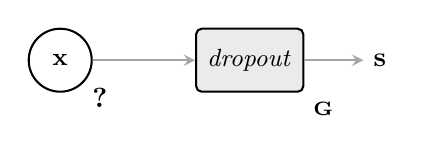
\begin{tikzpicture}[node distance=0.9cm and 1.3cm]
        \node[cgvar] (X) {$\mathbf{x}$};
        \node[cgopw, right=of X] (dp) {\textit{dropout}};
        \node[right=of dp, xshift=-0.55cm] (S) {$\mathbf{s}$};
        \draw[cgedge] (X) -- (dp);
        \draw[cgedge] (dp) -- (S);
        \node[cggrad, below right=0.05cm and 0.05cm of dp] {$\mathbf{G}$};
        \node[cggrad, below right=0.0cm and 0.05cm of X, font=\normalsize\bfseries] {?};
    \end{tikzpicture}
    \end{center}

    Em uma iteração com $d = 4$ temos
    \[
    \mathbf{x} = (2;\ -1;\ 3;\ 0{,}5), \qquad
    \mathbf{u} = (1;\ 0;\ 1;\ 1), \qquad
    \mathbf{G} = \frac{\partial J}{\partial \mathbf{s}} = (4;\ 6;\ -2;\ 8).
    \]
    Qual é o gradiente $\partial J / \partial \mathbf{x}$ que o nodo de \textit{dropout} envia pela sua aresta de entrada?

    \begin{enumerate}[(a)]
        \item $(4;\ 6;\ -2;\ 8)$
        \item $(8;\ -6;\ -6;\ 4)$
        \item $(2;\ 0;\ 3;\ 0{,}5)$
        \item $(0;\ 6;\ 0;\ 0)$
        \item $(1;\ 0;\ 1;\ 1)$
        \item $(8;\ 0;\ -6;\ 4)$
        \item $(4;\ 0;\ -2;\ 8)$
        \item $(0;\ 0;\ 0;\ 0)$
    \end{enumerate}
    %g

    \item Um classificador com três classes produz os \textit{logits} $\mathbf{z} = \begin{bmatrix} 1 & 3 & 1 \end{bmatrix}$ para uma instância cuja classe correta é a primeira. A saída passa por uma SoftMax e o custo é a entropia cruzada. Considere também duas modificações dos \textit{logits}: \textbf{(A)} somar $5$ a todos os componentes, obtendo $\begin{bmatrix} 6 & 8 & 6 \end{bmatrix}$, e \textbf{(B)} multiplicar todos os componentes por $2$, obtendo $\begin{bmatrix} 2 & 6 & 2 \end{bmatrix}$. Use $e^{2} \approx 7{,}39$, $e^{4} \approx 54{,}60$, $\ln 9{,}39 \approx 2{,}24$ e $\ln 56{,}60 \approx 4{,}04$. Quais são os valores da entropia cruzada para os \textit{logits} originais, para (A) e para (B), nessa ordem?

    \begin{enumerate}[(a)]
        \item $2{,}24$; $2{,}24$; $4{,}04$
        \item $2{,}24$; $7{,}24$; $4{,}04$
        \item $2{,}24$; $2{,}24$; $2{,}24$
        \item $2{,}24$; $2{,}24$; $4{,}48$
        \item $2{,}24$; $7{,}24$; $4{,}48$
        \item $2{,}24$; $7{,}24$; $2{,}24$
        \item $2{,}24$; $2{,}24$; $1{,}12$
        \item $2{,}24$; $7{,}24$; $1{,}12$
    \end{enumerate}
    %a

\end{enumerate}

\newpage

\subsection*{Gabarito}
\color{blue}
\begin{enumerate}[1)]

    \item a. A regra da cadeia local exige apenas o gradiente \textit{upstream}, que resume todo o caminho da \textit{loss} até a saída do nodo, e a derivada local da operação do nodo em relação a cada entrada. Essa localidade é o que torna o \textit{backpropagation} eficiente. A alternativa (b) descreve diferenciação simbólica e (c) descreve diferenças finitas, métodos que a diferenciação automática substitui; (d) inverte a lógica, pois os gradientes dos parâmetros são o resultado do percurso, não um pré-requisito.

    \item c. \textit{Forward}: $u = 3$, $v = 6$, $f = 18$. No \textit{backward}, $b$ recebe contribuição por dois caminhos: via $u$, $\frac{\partial f}{\partial u} \cdot 1 = v = 6$; via $v$, $\frac{\partial f}{\partial v} \cdot c = u \cdot c = 9$. Somando, $\frac{\partial f}{\partial b} = 6 + 9 = 15$. Os distratores $6$ e $9$ são os caminhos isolados e $18$ é o valor do \textit{forward}. Verificação analítica: com $a=1$ e $c=3$, $f(b) = 3b + 3b^2$ e $f'(2) = 3 + 12 = 15$.

    \item
    \begin{enumerate}[a)]
        \item \textit{Forward pass}, na ordem topológica:
        \begin{align*}
            u &= a + b = 2 + 3 = 5\\
            v &= \max(b, c) = \max(3, 4) = 4\\
            f &= u \cdot v = 5 \cdot 4 = 20
        \end{align*}
        \item \textit{Backward pass}, iniciando com $\partial f/\partial f = 1$ e percorrendo o grafo na ordem inversa:
        \begin{itemize}
            \item Nodo $f = u \cdot v$ (comutador): cada entrada recebe o gradiente \textit{upstream} multiplicado pelo valor da outra entrada, logo $\frac{\partial f}{\partial u} = 1 \cdot v = 4$ e $\frac{\partial f}{\partial v} = 1 \cdot u = 5$.
            \item Nodo $u = a + b$ (distribuidor): copia o gradiente \textit{upstream} para as duas entradas, logo $\frac{\partial f}{\partial a} = 4$ e a contribuição para $b$ por este caminho é $4$.
            \item Nodo $v = \max(b, c)$ (roteador): como $c = 4 > b = 3$, a entrada vencedora é $c$, que recebe o gradiente inteiro, $\frac{\partial f}{\partial c} = 5$. A contribuição para $b$ por este caminho é $0$.
            \item Variável $b$ usada em dois nodos (somador no \textit{backward}): os gradientes que chegam são somados, $\frac{\partial f}{\partial b} = 4 + 0 = 4$.
        \end{itemize}
        Resultado: $\frac{\partial f}{\partial a} = 4$, $\frac{\partial f}{\partial b} = 4$ e $\frac{\partial f}{\partial c} = 5$. Verificação: na região em que $c > b$ vale $f = (a+b)\,c$, portanto $\frac{\partial f}{\partial a} = c = 4$, $\frac{\partial f}{\partial b} = c = 4$ e $\frac{\partial f}{\partial c} = a + b = 5$.
    \end{enumerate}

    \item
    \begin{enumerate}[a)]
        \item Decomposição em nodos elementares, na ordem do \textit{forward}:
        \begin{align*}
            t_1 &= \theta_1 \cdot x_1 \quad (\text{produto})\\
            t_2 &= \theta_2 \cdot x_2 \quad (\text{produto})\\
            s_1 &= \theta_0 + t_1 \quad (\text{soma})\\
            z &= s_1 + t_2 \quad (\text{soma})\\
            \hat{y} &= \sigma(z) \quad (\text{sigmoide agrupada})\\
            L &= -\left(y\ln\hat{y} + (1-y)\ln(1-\hat{y})\right) \quad (\textit{loss})
        \end{align*}
        \item \textit{Backward pass} nodo a nodo, iniciando com $\partial L/\partial L = 1$:
        \begin{itemize}
            \item Nodo da \textit{loss}: derivando $L$ em relação a $\hat{y}$,
            $$\frac{\partial L}{\partial \hat{y}} = -\frac{y}{\hat{y}} + \frac{1-y}{1-\hat{y}} = \frac{\hat{y} - y}{\hat{y}(1-\hat{y})}.$$
            \item Nodo sigmoide: a derivada local é $\sigma'(z) = \hat{y}(1-\hat{y})$, então
            $$\frac{\partial L}{\partial z} = \frac{\partial L}{\partial \hat{y}} \cdot \hat{y}(1-\hat{y}) = \frac{\hat{y} - y}{\hat{y}(1-\hat{y})} \cdot \hat{y}(1-\hat{y}) = \hat{y} - y.$$
            \item Nodos de soma (distribuidores): copiam $\hat{y} - y$ para todas as entradas, logo
            $$\frac{\partial L}{\partial s_1} = \frac{\partial L}{\partial t_2} = \frac{\partial L}{\partial \theta_0} = \frac{\partial L}{\partial t_1} = \hat{y} - y.$$
            \item Nodos de produto (comutadores): multiplicam o gradiente \textit{upstream} pelo valor da outra entrada, logo
            $$\frac{\partial L}{\partial \theta_1} = (\hat{y} - y)\,x_1 \quad \text{e} \quad \frac{\partial L}{\partial \theta_2} = (\hat{y} - y)\,x_2.$$
        \end{itemize}
        Resumo: $\frac{\partial L}{\partial \theta_0} = \hat{y} - y$, $\frac{\partial L}{\partial \theta_1} = (\hat{y} - y)\,x_1$ e $\frac{\partial L}{\partial \theta_2} = (\hat{y} - y)\,x_2$. A simplificação ocorre porque o denominador $\hat{y}(1-\hat{y})$ da derivada da BCE cancela exatamente com a derivada da sigmoide, deixando o gradiente na pré-ativação igual ao erro $\hat{y} - y$.
    \end{enumerate}

    \item O \textit{backward pass} é a aplicação repetida da regra da cadeia sobre uma composição de operações elementares. Para automatizar esse processo, o \textit{framework} precisa saber quais operações foram executadas e em que ordem de dependência, e é exatamente isso que o grafo (um DAG) registra: cada operação executada no \textit{forward} vira um nodo, e as arestas indicam de quais valores cada nodo depende. Com o grafo montado, basta percorrê-lo na ordem topológica inversa multiplicando o gradiente \textit{upstream} pela derivada local de cada nodo, o que é eficiente no caso típico de redes neurais, com uma \textit{loss} escalar e muitos parâmetros.

    Durante o \textit{forward pass}, três coisas precisam ser armazenadas: (1) a estrutura do grafo, ou seja, quais nodos alimentam quais, pois sem ela não há como saber para onde propagar cada gradiente; (2) a operação realizada em cada nodo, pois cada operação elementar conhece a própria regra de derivada local; (3) os valores intermediários calculados no \textit{forward} que as derivadas locais consomem. Exemplos do item (3): o nodo de produto $z = x \cdot y$ precisa guardar os valores das entradas, pois no \textit{backward} cada entrada recebe o gradiente multiplicado pelo valor da outra ($\partial z/\partial x = y$ e $\partial z/\partial y = x$); o nodo sigmoide precisa guardar a própria saída, pois $\sigma'(z) = \sigma(z)(1 - \sigma(z))$; o nodo de máximo precisa registrar qual entrada venceu para rotear o gradiente inteiro para ela.

    \item a. Com $\mathbf{Z} = \mathbf{A}\,\mathbf{\Theta}^{\top}$, o nodo \textit{matmul} segue a mesma regra do nodo $\times$ escalar: cada entrada recebe o gradiente \textit{upstream} multiplicado pela outra entrada, com as transpostas ajustando as dimensões. Conferindo: $\mathbf{G}\,\mathbf{\Theta}$ é $(N\times d_s)(d_s\times d_e) = N\times d_e$, a forma de $\mathbf{A}$, e $\mathbf{G}^{\top}\mathbf{A}$ é $(d_s\times N)(N\times d_e) = d_s\times d_e$, a forma de $\mathbf{\Theta}$. A alternativa (b) aplica a regra do produto sem transposta $\mathbf{C} = \mathbf{A}\mathbf{B}$, ignorando a convenção $\mathbf{Z} = \mathbf{A}\,\mathbf{\Theta}^{\top}$, e produz até uma multiplicação indefinida ($\mathbf{G}\,\mathbf{\Theta}^{\top}$ tenta multiplicar $N\times d_s$ por $d_e\times d_s$); em (c) as duas expressões estão trocadas e nenhuma tem a forma da entrada correspondente; em (d) nenhuma das multiplicações é definida em geral.

    \item
    \begin{enumerate}[a)]
        \item \textit{Forward pass}, nodo a nodo:
        \begin{align*}
            \mathbf{Z}^{(1)} &= \mathbf{X}{\mathbf{\Theta}^{(1)}}^{\top} = \begin{bmatrix} 1 & 2 \end{bmatrix}\begin{bmatrix} 0.5 & 0.5 \\ -0.5 & 0.5 \end{bmatrix} = \begin{bmatrix} -0.5 & 1.5 \end{bmatrix}\\
            \mathbf{A}^{(1)} &= \sigma(\mathbf{Z}^{(1)}) = \begin{bmatrix} 0.3775 & 0.8176 \end{bmatrix}\\
            \mathbf{Z}^{(2)} &= \mathbf{A}^{(1)}{\mathbf{\Theta}^{(2)}}^{\top} = 0.5 \cdot 0.3775 - 0.5 \cdot 0.8176 = -0.2200\\
            \hat{y} &= \sigma(-0.2200) = 0.4452\\
            J &= \tfrac{1}{2}(1 - 0.4452)^{2} = 0.1539
        \end{align*}
        \item \textit{Backward pass}, iniciando com $\partial J/\partial J = 1$:
        \begin{itemize}
            \item Nodo \textit{loss}: $\frac{\partial J}{\partial \hat{y}} = \hat{y} - y = -0.5548$.
            \item Nodo sigmoide da saída: $\boldsymbol{\delta}^{(2)} = \frac{\partial J}{\partial \hat{y}} \odot \hat{y}(1-\hat{y}) = -0.5548 \cdot 0.2470 = -0.1370$.
            \item Nodo \textit{matmul} da camada 2: $\frac{\partial J}{\partial \mathbf{\Theta}^{(2)}} = {\boldsymbol{\delta}^{(2)}}^{\top}\mathbf{A}^{(1)} = \begin{bmatrix} -0.0517 & -0.1120 \end{bmatrix}$ e $\frac{\partial J}{\partial \mathbf{A}^{(1)}} = \boldsymbol{\delta}^{(2)}\mathbf{\Theta}^{(2)} = \begin{bmatrix} -0.0685 & 0.0685 \end{bmatrix}$.
            \item Nodo sigmoide da camada oculta: $\boldsymbol{\delta}^{(1)} = \frac{\partial J}{\partial \mathbf{A}^{(1)}} \odot \mathbf{A}^{(1)} \odot (1 - \mathbf{A}^{(1)}) = \begin{bmatrix} -0.0685 & 0.0685 \end{bmatrix} \odot \begin{bmatrix} 0.2350 & 0.1491 \end{bmatrix} = \begin{bmatrix} -0.0161 & 0.0102 \end{bmatrix}$.
            \item Nodo \textit{matmul} da camada 1: $\frac{\partial J}{\partial \mathbf{\Theta}^{(1)}} = {\boldsymbol{\delta}^{(1)}}^{\top}\mathbf{X} = \begin{bmatrix} -0.0161 \\ 0.0102 \end{bmatrix}\begin{bmatrix} 1 & 2 \end{bmatrix} = \begin{bmatrix} -0.0161 & -0.0322 \\ 0.0102 & 0.0204 \end{bmatrix}$.
        \end{itemize}
        $\mathbf{X}$ e $y$ são dados do problema, então não recebem gradiente.
    \end{enumerate}

    \item g. O \textit{dropout} é um nodo \textbf{elemento a elemento}, como a ReLU, e não um nodo que mistura posições, como o \textit{matmul}. Para nodos desse tipo o \textit{backward} é a regra escalar aplicada posição a posição: multiplica-se o gradiente \textit{upstream} pela derivada local. Como $s_i = u_i\,x_i$ e $u_i$ é uma constante no \textit{backward} (foi sorteada no \textit{forward} e não é um parâmetro treinável), a derivada local é
    \[
    \frac{\partial s_i}{\partial x_i} = u_i \in \{0, 1\},
    \qquad\text{logo}\qquad
    \frac{\partial J}{\partial \mathbf{x}} = \mathbf{G} \odot \mathbf{u}.
    \]
    A máscara age como uma \emph{chave}: nas posições sorteadas com $u_i = 1$ o gradiente passa intacto, e nas posições com $u_i = 0$ ele é zerado, exatamente como a unidade desligada não contribuiu para a saída no \textit{forward}. Substituindo,
    \[
    \frac{\partial J}{\partial \mathbf{x}} = (4;\ 6;\ -2;\ 8) \odot (1;\ 0;\ 1;\ 1) = (4;\ 0;\ -2;\ 8).
    \]
    Note o paralelo com a ReLU exibida no enunciado: lá a derivada local é $\mathrm{ReLU}'(\mathbf{Z})$, que também vale $1$ ou $0$ por posição. O \textit{dropout} tem a mesma estrutura, com a diferença de que quem decide entre $1$ e $0$ é a máscara sorteada, e não o sinal da pré-ativação. Em (a), $\mathbf{G}$ é repassado intacto, tratando o \textit{dropout} como nodo de soma (\textit{distribuidor}) e ignorando a máscara; em (b), a regra do \textit{matmul} é aplicada à entrada errada, usando $\mathbf{G} \odot \mathbf{x}$, quando o ``outro fator'' do produto é $\mathbf{u}$; (c) devolve $\mathbf{u} \odot \mathbf{x}$, que é a \emph{saída} do nodo no \textit{forward}, não o gradiente; (d) usa a máscara invertida $\mathbf{1} - \mathbf{u}$, deixando passar gradiente exatamente nas posições que foram desligadas; (e) devolve a derivada local $\mathbf{u}$ isolada, esquecendo de multiplicar pelo gradiente \textit{upstream}; (f) combina os dois erros anteriores, calculando $\mathbf{G} \odot \mathbf{x} \odot \mathbf{u}$; (h) zera o gradiente inteiro por supor que um nodo com componente aleatória bloqueia a retropropagação, mas a máscara, embora aleatória, é uma constante conhecida no \textit{backward} e o caminho até $\mathbf{x}$ continua diferenciável.

    \item a. Com classe correta $1$, a entropia cruzada é $-\ln \mathrm{softmax}(\mathbf{z})_1 = -z_1 + \ln\sum_j e^{z_j}$. \textbf{Original:} $-1 + \ln(e^1 + e^3 + e^1) = -1 + 1 + \ln(2 + e^{2}) = \ln 9{,}39 \approx 2{,}24$. \textbf{(A):} somar a mesma constante $c$ a todos os \textit{logits} multiplica numerador e denominador da SoftMax por $e^{c}$, então as probabilidades e o custo não mudam: $2{,}24$. É exatamente a propriedade que o truque do log-sum-exp explora. \textbf{(B):} $-2 + \ln(2e^{2} + e^{6}) = \ln(2 + e^{4}) = \ln 56{,}60 \approx 4{,}04$. Multiplicar os \textit{logits} por $2$ aumenta a diferença entre a classe errada ($z_2$) e a correta, a SoftMax fica mais confiante na classe errada e o custo cresce, mas sem dobrar. O segundo valor distingue quem sabe que a SoftMax é invariante a deslocamentos ($2{,}24$) de quem soma a constante ao custo ($7{,}24$), como se a entropia cruzada fosse linear nos \textit{logits}. O terceiro valor distingue o resultado correto ($4{,}04$) de três erros sobre a mudança de escala: supor que a SoftMax também é invariante a ela ($2{,}24$), tratar $\ln\sum_j e^{2z_j}$ como $2\ln\sum_j e^{z_j}$ e dobrar o custo ($4{,}48$), ou dividi-lo por dois ($1{,}12$), invertendo o efeito de aumentar a escala. Assim, (b) erra o deslocamento e acerta a escala; (c), (d) e (g) acertam o deslocamento e erram a escala (invariância, dobro e metade, respectivamente); (e), (f) e (h) erram as duas modificações.
\end{enumerate}

\end{document}
